\chapter*{Практика 2. Помехоустойчивое кодирование}
\addcontentsline{toc}{chapter}{Практика 2. Помехоустойчивое кодирование}
\label{ch:2_practice}

\textit{\textbf{Задание:}} Реализовать операцию свёрточного кодирования и витербидекодирования битового сообщения.

\begin{itemize}
    \item Реализован сверточный кодер с параметрами:
    \begin{itemize}
        \item Порождающие полиномы G1=171, G2=133 (восьмеричные)
        \item Длина кодового ограничения $k=7$
    \end{itemize}
    \item Разработан декодер Витерби:
    \begin{itemize}
        \item Реализован алгоритм поиска оптимального пути
        \item Вычисление метрик пути
        \item Обратное прослеживание для восстановления исходной последовательности
    \end{itemize}
\end{itemize}

\begin{figure}[ht]
    \centering
    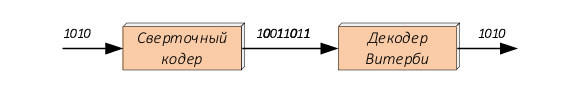
\includegraphics[width=0.8\textwidth]{convolutional_encoder_decoder.png}
    \caption{Блоксхема работы свёрточного кодера и декодера Витерби}
    \label{fig:convolutional_encoder_decoder}
\end{figure}

\begin{figure}[ht]
    \centering
    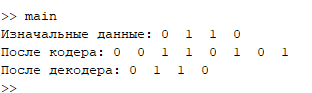
\includegraphics[width=0.8\textwidth]{2practice_result.png}
    \caption{Результат второй практики}
    \label{fig:2practice_result}
\end{figure}